\section[Co je AI]{Co je umělá inteligence}

% ----------------------------------------------------------------------------

\begin{frame}{Ne-definice}

    \begin{center}
        \Large
    \textbf{Umělá inteligence} = obor informatiky, který se zabývá řešením
    úloh\ldots
    \end{center}

    \vspace{10pt}

    \begin{itemize}

        \item<2-> O kterých se vágně shodneme, že k~jejich řešení lidé potřebují
            inteligenci

        \item<3-> Někdy úlohy, které vyžadují \textbf{velké mentální úsilí} \\
            \quad \emph{hraní šachů nebo Go, automatický překlad}

        \item<4-> Někdy úlohy, které jsou \textbf{pro člověka triviální} \\
            \quad \emph{rozpoznávání objektů na fotografii, rozpozávání řeči}

    \end{itemize}

    \centering\vspace{15pt}

    \visible<5->{Hranice, co se považuje AI, se posouvá sem a tam\ldots}

\end{frame}

% ----------------------------------------------------------------------------

\begin{frame}{Exponenicálně rostoucí obor}

    \centering
    \includegraphics[scale=.25]{./img/exp_growth.jpg}

    Počet publikovaných článeků se každé dva roky zdvojnásobí.

    {\footnotesize Zdroj: \citet{krenn2022prediction}}

\end{frame}

% ----------------------------------------------------------------------------

\begin{frame}{Společensko-vědní pohled}

    \begin{quote}
        [T]he phrase “artificial intelligence” is deployed when the people building
        or selling a particular set of technologies will profit from getting others
        to believe that their technology is similar to humans, able to do things
        that, in fact, intrinsically require human judgment, perception, or
        creativity.
    \end{quote}

    {\footnotesize Zdroj: \citet{bender2025ai}}

\end{frame}

% ----------------------------------------------------------------------------

\begin{frame}{Inteligentní chování = AI?}

    \begin{columns}
        \column{.40\textwidth}
        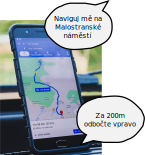
\includegraphics[scale=0.45]{./img/navigation.pdf}

        \column{.55\textwidth}

        \begin{enumerate}

            \item<2-> Rozpoznávání řeči \\
                \visible<9->{\hfill\it\color{gray} neuronová síť naučená z nahrávek}

            \item<3-> Analýza textu \\
                \visible<10->{\hfill\it\color{gray} pravidla nebo neuronová síť}

            \item<4-> Vyhledání cíle na mapě \\
                \visible<11->{\hfill\it\color{gray} vyhledávání v databázi, spíš SW inženýrství}

            \item<5-> Nalezení nejlepší cesty \\
                \visible<12->{\hfill\it\color{gray} optimalizace, diskrétní matematika}

            \item<6-> Určení polohy, rozhodnutí co je další krok na nejlepší cestě
                \visible<13->{\hfill\it\color{gray} jednoduchý algoritmus}

            \item<7-> Generování přirozeného jazyka \\
                \visible<14->{\hfill\it\color{gray} jednoduchý algoritmus nebo neuronová síť}

            \item<8-> Syntéza řeči \\
                \visible<15->{\hfill\it\color{gray} neuronová síť naučená z nahrávek}

        \end{enumerate}

    \end{columns}

\end{frame}

% ----------------------------------------------------------------------------

\begin{frame}{Strong vs. Weak AI}

    \begin{columns}[t]
        \column{.45\textwidth}
        \begin{center}
        \visible<1->{{\Large \textbf{Strong AI}}}
        \end{center}

        \vspace{5pt}

        \begin{itemize}

            \item<2-> Také AGI -- \\ \quad Artifitial General Inteligence

            \item<3-> Cílem je obecně \textbf{inteligentní stroj}, který v důsledku
			    toho umí řešit \textbf{všechny úlohy}

            \item<4-> (Ne)vědecký/(ne)inženýrský koncept

        \end{itemize}


        \column{.45\textwidth}
        \begin{center}
        \visible<5->{{\Large \textbf{Weak AI}}}
        \end{center}

        \vspace{5pt}

        \begin{itemize}

            \item<6-> Také Narrow AI

            \item<7-> Cílem je řešit \textbf{jednotlivé úlohy}, které vyžadují
					(lidskou) inteligenci

            \item<8-> Všechno, o čem bude dnes řeč, je weak AI

        \end{itemize}

		\vspace{15pt}

			\visible<9->{Co je inteligence a co je jenom počítání?}

    \end{columns}


\end{frame}

% ----------------------------------------------------------------------------

\begin{frame}{Superintelligence: Pojem inteligence je problematický}

    \begin{itemize}

        \item<1-> Moderní pojetí inteligence jako jedné měřitelné veličiny vzniklo
            z velké části v kontextu \textbf{eugenického hnutí} (konec 19. a začátek 20. století)

            \begin{itemize}
                \item<2-> Eugenici potřebovali lidi \emph{seřadit} -- nutně tedy
                    jednodimenzionální škála
                \item<3-> IQ testy často sloužily jako nástroj k odůvodnění
                    sociální nerovnosti
            \end{itemize}

        \item<4-> Skutečná lidská inteligence je \textbf{mnohodimenzionální}

            \begin{itemize}
                \item<5-> Gardnerova teorie mnohočetných inteligencí \\
                    \quad {\small\it jazyková, logická, prostorová, hudební, tělesná\ldots}
                \item<6-> Sternbergův triarchický model \\
                    \quad {\small\it analytická, kreativní, praktická}
            \end{itemize}

        \item<7-> Říct, že někdo nebo něco je „inteligentnější", \textbf{nedává
            jednoznačný smysl}

            \begin{itemize}
                \item<8-> Inteligentnější \emph{v čem} a \emph{pro jaký účel}?
                \item<9-> Šachový program poráží každého velmistra~-- je tedy
                    „inteligentnější než člověk"?
            \end{itemize}

    \end{itemize}

\end{frame}


% ----------------------------------------------------------------------------

%\begin{frame}{Strong AI: Turingův test}
%
%\end{frame}
%
%% ----------------------------------------------------------------------------
%
%\begin{frame}{Strong AI: Čínský pokoj}
%
%\end{frame}

% ----------------------------------------------------------------------------

\begin{frame}{Když se dneska řekne AI}

    \Large

    \begin{itemize}[<+->]

        \item Většinou jsou to metody založené na \textbf{strojovém učení}  \\  \quad a zpracování
            \textbf{hodně dat} \\[1em]

        \item Často je to strojové učení pomocí \textbf{neuronových sítí} \\[1em]

        \item Fantazie/marketing CEOs technologických firem a hype médií
            \visible<4->{\hfill\it\color{gray} (a někdy i vědců)} \\[1em]

    \end{itemize}


\end{frame}
